
%(BEGIN_QUESTION)
% Copyright 2011, Tony R. Kuphaldt, released under the Creative Commons Attribution License (v 1.0)
% This means you may do almost anything with this work of mine, so long as you give me proper credit

This pressure-control system does not appear to be regulating water pressure correctly.  The SP is set for 110 PSI (out of a 0-150 PSI range), but the PV display on the controller faceplate registers only 27 PSI, and has for quite a while.  You happen to notice that the controller output reads 38\% on the faceplate:

$$\includegraphics[width=15.5cm]{i00338x01.eps}$$

Your first test is to measure loop current in the circuit connecting the pressure transmitter to the pressure controller.  There, your multimeter registers 6.88 milliamps.  Your next step is to record the pressure gauge's indication (at the I/P output tube): 7.5 PSI.

\vskip 10pt

Identify the likelihood of each specified fault for this control system.  Consider each fault one at a time (i.e. no coincidental faults), determining whether or not each fault could independently account for {\it all} measurements and symptoms in this circuit.

% No blank lines allowed between lines of an \halign structure!
% I use comments (%) instead, so that TeX doesn't choke.

$$\vbox{\offinterlineskip
\halign{\strut
\vrule \quad\hfil # \ \hfil & 
\vrule \quad\hfil # \ \hfil & 
\vrule \quad\hfil # \ \hfil \vrule \cr
\noalign{\hrule}
%
% First row
{\bf Fault} & {\bf Possible} & {\bf Impossible} \cr
%
\noalign{\hrule}
%
% Another row
PT out of calibration (outputting wrong current) &  &  \cr
%
\noalign{\hrule}
%
% Another row
PIC input out of calibration (not interpreting PV signal properly) &  &  \cr
%
\noalign{\hrule}
%
% Another row
PIC output out of calibration (not sending correct mA signal to I/P) &  &  \cr
%
\noalign{\hrule}
%
% Another row
Pressure gauge out of calibration (not displaying pressure properly) &  &  \cr
%
\noalign{\hrule}
%
% Another row
I/P out of calibration (not outputting correct pressure) &  &  \cr
%
\noalign{\hrule}
%
% Another row
Control valve is oversized &  &  \cr
%
\noalign{\hrule}
%
% Another row
Control valve is undersized &  &  \cr
%
\noalign{\hrule}
%
% Another row
PIC is poorly tuned (not making good control ``decisions'') &  &  \cr
%
\noalign{\hrule}
%
% Another row
Instrument air supply not at full pressure &  &  \cr
%
\noalign{\hrule}
} % End of \halign 
}$$ % End of \vbox

\underbar{file i00338}
%(END_QUESTION)





%(BEGIN_ANSWER)

This is a graded question -- no answers or hints given!

%(END_ANSWER)





%(BEGIN_NOTES)

A good diagnostic principle to apply here is that of {\it correspondence}: check for which variables properly correspond with each other, and which do not.  Clearly, the 110 PSI setpoint entered into the controller is nowhere near the PV value displayed by the controller (27 PSI).

If we take the measured milliamp signal (6.88 mA) and convert that into a corresponding pressure given the transmitter's range of 0 to 150 PSI, we may compare this calculated pressure value against the controller's display to see if they agree.  In this case, 6.88 mA is equivalent to 27 PSI, which agrees with the controller display.  From this we may conclude that the controller input and display are not at fault, because the controller is receiving a current signal equivalent to 27 PSI and that is what it is displaying.  

Next, we can check to see that the I/P converter's output signal of 7.5 PSI corresponds with the controller's output display of 38\%.  Indeed this is the case (38\% = 7.56 PSI in a 3-15 PSI range).  Thus, things appear to be okay from the controller output display through the I/P converter and the pressure gauge.

The real question, however, is why the controller isn't trying harder to raise the pressure to setpoint, since the output shows 38\% (far from a shut drain valve).  If the controller were doing its job properly, we would expect to see it shut the valve completely in an effort to raise the filter pressure.  Since it isn't doing this, we may conclude something is wrong with the controller's tuning (or perhaps it is in manual mode).


% No blank lines allowed between lines of an \halign structure!
% I use comments (%) instead, so that TeX doesn't choke.

$$\vbox{\offinterlineskip
\halign{\strut
\vrule \quad\hfil # \ \hfil & 
\vrule \quad\hfil # \ \hfil & 
\vrule \quad\hfil # \ \hfil \vrule \cr
\noalign{\hrule}
%
% First row
{\bf Fault} & {\bf Possible} & {\bf Impossible} \cr
%
\noalign{\hrule}
%
% Another row
PT out of calibration (outputting wrong current) &  & $\surd$ \cr
%
\noalign{\hrule}
%
% Another row
PIC input out of calibration (not interpreting PV signal properly) &  & $\surd$ \cr
%
\noalign{\hrule}
%
% Another row
PIC output out of calibration (not sending correct mA signal to I/P) &  & $\surd$ \cr
%
\noalign{\hrule}
%
% Another row
Pressure gauge out of calibration (not displaying pressure properly) &  & $\surd$ \cr
%
\noalign{\hrule}
%
% Another row
I/P out of calibration (not outputting correct pressure) &  & $\surd$ \cr
%
\noalign{\hrule}
%
% Another row
Control valve is oversized &  & $\surd$ \cr
%
\noalign{\hrule}
%
% Another row
Control valve is undersized &  & $\surd$ \cr
%
\noalign{\hrule}
%
% Another row
PIC is poorly tuned (not making good control ``decisions'') & $\surd$ &  \cr
%
\noalign{\hrule}
%
% Another row
Instrument air supply not at full pressure &  & $\surd$ \cr
%
\noalign{\hrule}
} % End of \halign 
}$$ % End of \vbox

%INDEX% Basics, control loop troubleshooting: determining cause of control problem

%(END_NOTES)


